
\documentclass[10pt]{beamer}

\title{Simulation Results}
\author{Ilija Nikolov, Lucas Z. Brito}
\institute{}
\date{2021}

\setbeamersize{text margin left=0.4cm, text margin right=0.4cm}
\begin{document}

\frame{\titlepage}
\begin{frame}
\frametitle{42correlated mixed dipD2}
Spin: 0.5,$B_0= 10$, $\gamma/2\pi = 4.0$,$\mathcal{H}=\text{I}_{z}+ b_D \big(3\cos^2\theta-1\big)I_{1z}I_{2z}.$$b_D\approx1.571$$theta\approx0.785$
\begin{columns}[T]
\begin{column}{.5\textwidth}
\begin{align*}
\rho_{\text{initial}}\doteq
\begin{pmatrix}
0.291 & 0.0 & 0.0 & 0.0 \\
0.0 & 0.309 & 0.0 & 0.0 \\
0.0 & 0.0 & 0.2 & 0.0 \\
0.0 & 0.0 & 0.0 & 0.2
\end{pmatrix}
\\
\rho_{\text{final}}\doteq
\begin{pmatrix}
0.291 & 0.0 & 0.001 & -0.0 \\
0.0 & 0.309 & -0.0 & 0.001 \\
0.001 & -0.0 & 0.2 & 0.0 \\
-0.0 & 0.001 & 0.0 & 0.2
\end{pmatrix}
\end{align*}
\begin{column}{.5\textwidth}
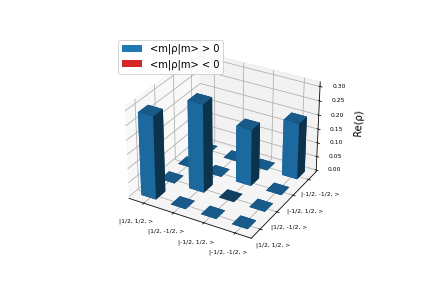
\includegraphics[width=1.5\textwidth]{./spin1-2/42correlated_mixed_dipD2/InitialRealPartDensityMatrix.png}
\end{column}
\begin{column}{.5\textwidth}
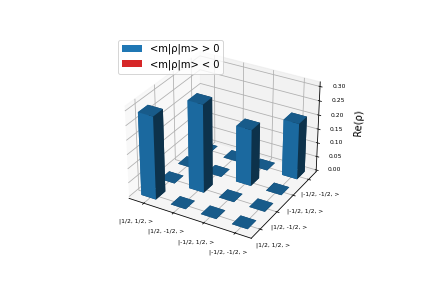
\includegraphics[width=1.5\textwidth]{./spin1-2/42correlated_mixed_dipD2/EvolvedRealPartDensityMatrix.png}
\end{column}
\end{column}
\begin{column}{.5\textwidth}
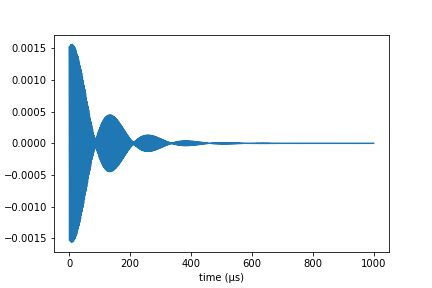
\includegraphics[width=\textwidth]{./spin1-2/42correlated_mixed_dipD2/FIDSignal.png}
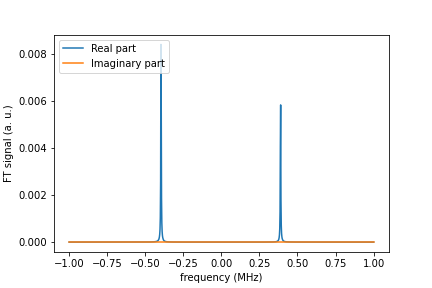
\includegraphics[width=\textwidth]{./spin1-2/42correlated_mixed_dipD2/FTSignal.png}
\end{column}
\end{columns}
\end{frame}
\begin{frame}
\frametitle{14uncorrelated mixed hyperfineAnisotrop}
Spin: 0.5,$B_0= 10$, $\gamma/2\pi = 4.0$,$\mathcal{H}=\text{I}_{z}+ \hat{S}\tilde{A}\hat{I}$$A=[[2, 0, 0], [0, 1, 0], [0, 0, 1]]$,
\begin{columns}[T]
\begin{column}{.5\textwidth}
\begin{align*}
\rho_{\text{initial}}\doteq
\begin{pmatrix}
0.213 & 0.0 & 0.0 & -0.025 \\
0.0 & 0.287 & -0.099 & 0.0 \\
0.0 & -0.099 & 0.287 & 0.0 \\
-0.025 & 0.0 & 0.0 & 0.213
\end{pmatrix}
\\
\rho_{\text{final}}\doteq
\begin{pmatrix}
0.213 & -0.0 & 0.0 & -0.025 \\
-0.0 & 0.287 & -0.099 & 0.0 \\
0.0 & -0.099 & 0.287 & -0.0 \\
-0.025 & 0.0 & -0.0 & 0.213
\end{pmatrix}
\end{align*}
\begin{column}{.5\textwidth}
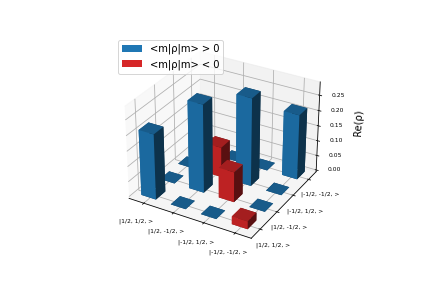
\includegraphics[width=1.5\textwidth]{./spin1-2/14uncorrelated_mixed_hyperfineAnisotrop/InitialRealPartDensityMatrix.png}
\end{column}
\begin{column}{.5\textwidth}
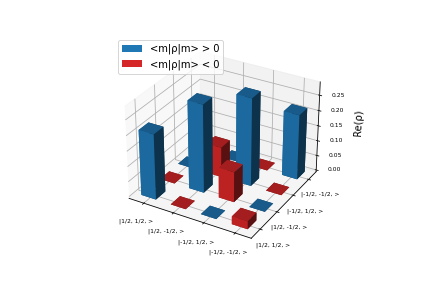
\includegraphics[width=1.5\textwidth]{./spin1-2/14uncorrelated_mixed_hyperfineAnisotrop/EvolvedRealPartDensityMatrix.png}
\end{column}
\end{column}
\begin{column}{.5\textwidth}
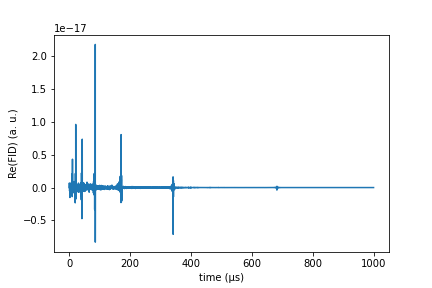
\includegraphics[width=\textwidth]{./spin1-2/14uncorrelated_mixed_hyperfineAnisotrop/FIDSignal.png}
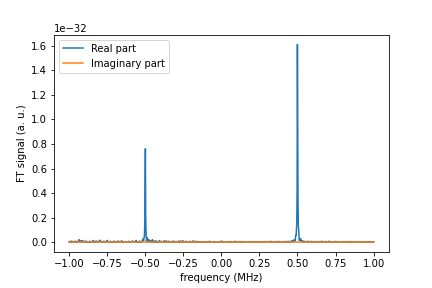
\includegraphics[width=\textwidth]{./spin1-2/14uncorrelated_mixed_hyperfineAnisotrop/FTSignal.png}
\end{column}
\end{columns}
\end{frame}
\begin{frame}
\frametitle{22uncorrelated pure dipD2}
Spin: 0.5,$B_0= 10$, $\gamma/2\pi = 4.0$,$\mathcal{H}=\text{I}_{z}+ b_D \big(3\cos^2\theta-1\big)I_{1z}I_{2z}.$$b_D\approx1.571$$theta\approx0.785$
\begin{columns}[T]
\begin{column}{.5\textwidth}
\begin{align*}
\rho_{\text{initial}}\doteq
\begin{pmatrix}
1.0 & 0.0 & 0.0 & 0.0 \\
0.0 & 0.0 & 0.0 & 0.0 \\
0.0 & 0.0 & 0.0 & 0.0 \\
0.0 & 0.0 & 0.0 & 0.0
\end{pmatrix}
\\
\rho_{\text{final}}\doteq
\begin{pmatrix}
1.0 & 0.0 & 0.008 & 0.0 \\
0.0 & 0.0 & 0.0 & 0.0 \\
0.008 & 0.0 & 0.0 & 0.0 \\
0.0 & 0.0 & 0.0 & 0.0
\end{pmatrix}
\end{align*}
\begin{column}{.5\textwidth}
\includegraphics[width=1.5\textwidth]{./spin1-2/22uncorrelated_pure_dipD2/InitialRealPartDensityMatrix.png}
\end{column}
\begin{column}{.5\textwidth}
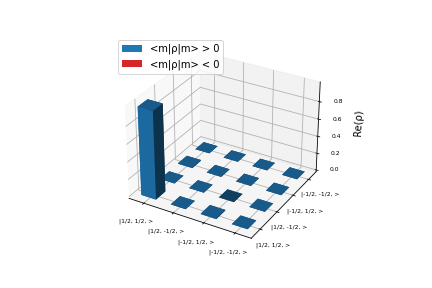
\includegraphics[width=1.5\textwidth]{./spin1-2/22uncorrelated_pure_dipD2/EvolvedRealPartDensityMatrix.png}
\end{column}
\end{column}
\begin{column}{.5\textwidth}
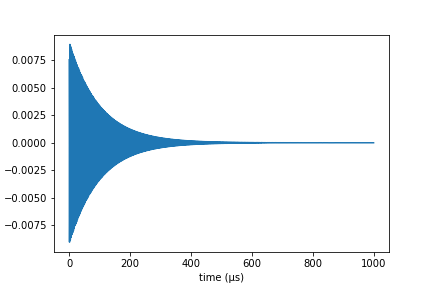
\includegraphics[width=\textwidth]{./spin1-2/22uncorrelated_pure_dipD2/FIDSignal.png}
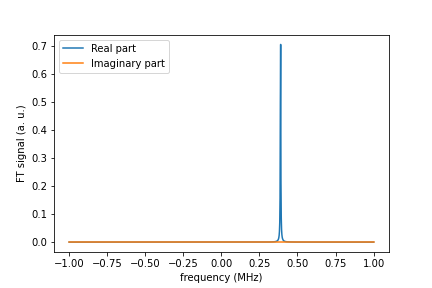
\includegraphics[width=\textwidth]{./spin1-2/22uncorrelated_pure_dipD2/FTSignal.png}
\end{column}
\end{columns}
\end{frame}
\begin{frame}
\frametitle{12uncorrelated mixed dipD2}
Spin: 0.5,$B_0= 10$, $\gamma/2\pi = 4.0$,$\mathcal{H}=\text{I}_{z}+ b_D \big(3\cos^2\theta-1\big)I_{1z}I_{2z}.$$b_D\approx1.571$$theta\approx0.785$
\begin{columns}[T]
\begin{column}{.5\textwidth}
\begin{align*}
\rho_{\text{initial}}\doteq
\begin{pmatrix}
0.453 & 0.0 & 0.0 & 0.0 \\
0.0 & 0.547 & 0.0 & 0.0 \\
0.0 & 0.0 & 0.0 & 0.0 \\
0.0 & 0.0 & 0.0 & 0.0
\end{pmatrix}
\\
\rho_{\text{final}}\doteq
\begin{pmatrix}
0.453 & 0.0 & 0.003 & 0.0 \\
0.0 & 0.547 & 0.0 & 0.004 \\
0.003 & 0.0 & 0.0 & 0.0 \\
0.0 & 0.004 & 0.0 & 0.0
\end{pmatrix}
\end{align*}
\begin{column}{.5\textwidth}
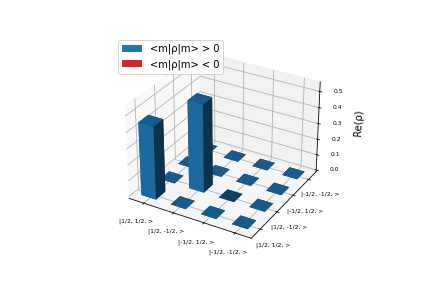
\includegraphics[width=1.5\textwidth]{./spin1-2/12uncorrelated_mixed_dipD2/InitialRealPartDensityMatrix.png}
\end{column}
\begin{column}{.5\textwidth}
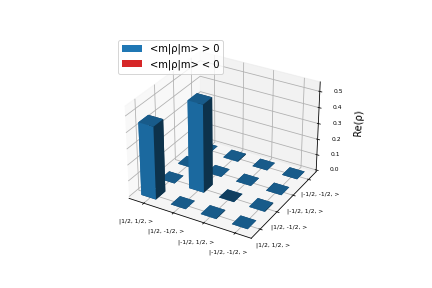
\includegraphics[width=1.5\textwidth]{./spin1-2/12uncorrelated_mixed_dipD2/EvolvedRealPartDensityMatrix.png}
\end{column}
\end{column}
\begin{column}{.5\textwidth}
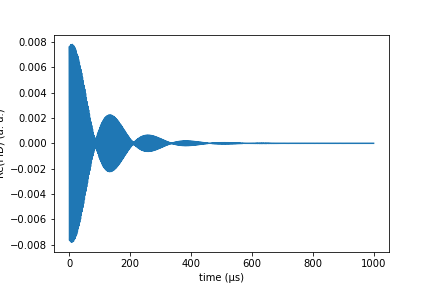
\includegraphics[width=\textwidth]{./spin1-2/12uncorrelated_mixed_dipD2/FIDSignal.png}
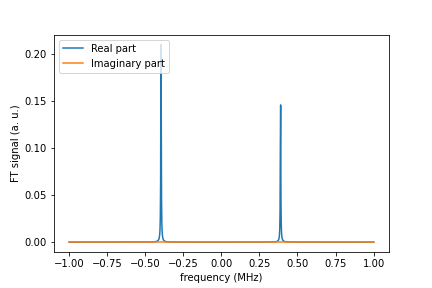
\includegraphics[width=\textwidth]{./spin1-2/12uncorrelated_mixed_dipD2/FTSignal.png}
\end{column}
\end{columns}
\end{frame}
\begin{frame}
\frametitle{13uncorrelated mixed hyperfine}
Spin: 0.5,$B_0= 10$, $\gamma/2\pi = 4.0$,$\mathcal{H}=\text{I}_{z}+ \hat{S}\tilde{A}\hat{I}$$A=[[1, 0, 0], [0, 1, 0], [0, 0, 1]]$,
\begin{columns}[T]
\begin{column}{.5\textwidth}
\begin{align*}
\rho_{\text{initial}}\doteq
\begin{pmatrix}
0.217 & 0.0 & 0.0 & 0.0 \\
0.0 & 0.283 & -0.067 & 0.0 \\
0.0 & -0.067 & 0.283 & 0.0 \\
0.0 & 0.0 & 0.0 & 0.217
\end{pmatrix}
\\
\rho_{\text{final}}\doteq
\begin{pmatrix}
0.217 & -0.0 & 0.0 & -0.0 \\
-0.0 & 0.283 & -0.067 & 0.0 \\
0.0 & -0.067 & 0.283 & -0.0 \\
-0.0 & 0.0 & -0.0 & 0.217
\end{pmatrix}
\end{align*}
\begin{column}{.5\textwidth}
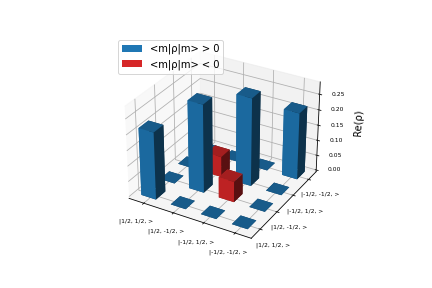
\includegraphics[width=1.5\textwidth]{./spin1-2/13uncorrelated_mixed_hyperfine/InitialRealPartDensityMatrix.png}
\end{column}
\begin{column}{.5\textwidth}
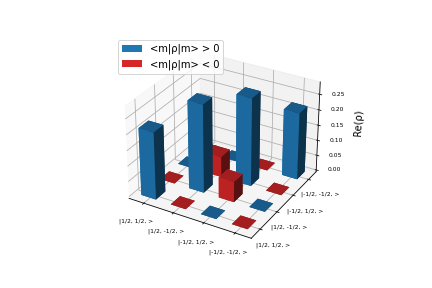
\includegraphics[width=1.5\textwidth]{./spin1-2/13uncorrelated_mixed_hyperfine/EvolvedRealPartDensityMatrix.png}
\end{column}
\end{column}
\begin{column}{.5\textwidth}
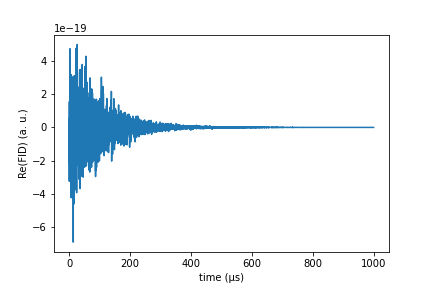
\includegraphics[width=\textwidth]{./spin1-2/13uncorrelated_mixed_hyperfine/FIDSignal.png}
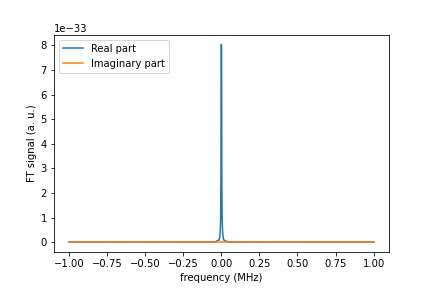
\includegraphics[width=\textwidth]{./spin1-2/13uncorrelated_mixed_hyperfine/FTSignal.png}
\end{column}
\end{columns}
\end{frame}
\begin{frame}
\frametitle{31correlated pure no interactions}
Spin: 0.5,$B_0= 10$, $\gamma/2\pi = 4.0$,$\mathcal{H}=\text{I}_{z}$
\begin{columns}[T]
\begin{column}{.5\textwidth}
\begin{align*}
\rho_{\text{initial}}\doteq
\begin{pmatrix}
0.5 & 0.0 & 0.5 & 0.0 \\
0.0 & 0.0 & 0.0 & 0.0 \\
0.5 & 0.0 & 0.5 & 0.0 \\
0.0 & 0.0 & 0.0 & 0.0
\end{pmatrix}
\\
\rho_{\text{final}}\doteq
\begin{pmatrix}
0.505 & 0.0 & 0.0 & 0.0 \\
0.0 & 0.0 & 0.0 & 0.0 \\
0.0 & 0.0 & 0.495 & 0.0 \\
0.0 & 0.0 & 0.0 & 0.0
\end{pmatrix}
\end{align*}
\begin{column}{.5\textwidth}
\includegraphics[width=1.5\textwidth]{./spin1-2/31correlated_pure_no_interactions/InitialRealPartDensityMatrix.png}
\end{column}
\begin{column}{.5\textwidth}
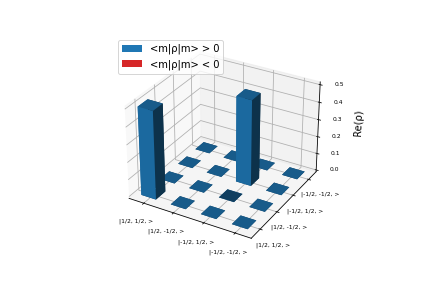
\includegraphics[width=1.5\textwidth]{./spin1-2/31correlated_pure_no_interactions/EvolvedRealPartDensityMatrix.png}
\end{column}
\end{column}
\begin{column}{.5\textwidth}
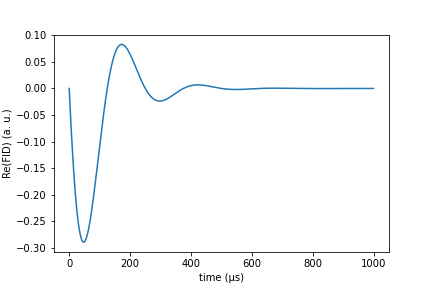
\includegraphics[width=\textwidth]{./spin1-2/31correlated_pure_no_interactions/FIDSignal.png}
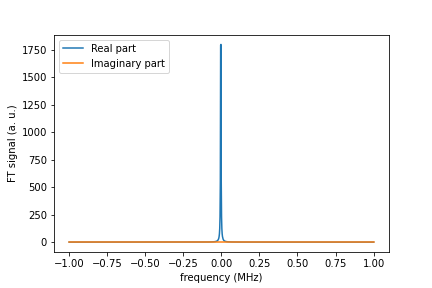
\includegraphics[width=\textwidth]{./spin1-2/31correlated_pure_no_interactions/FTSignal.png}
\end{column}
\end{columns}
\end{frame}
\begin{frame}
\frametitle{33correlated pure hyperfine}
Spin: 0.5,$B_0= 10$, $\gamma/2\pi = 4.0$,$\mathcal{H}=\text{I}_{z}+ \hat{S}\tilde{A}\hat{I}$$A=[[1, 0, 0], [0, 1, 0], [0, 0, 1]]$,
\begin{columns}[T]
\begin{column}{.5\textwidth}
\begin{align*}
\rho_{\text{initial}}\doteq
\begin{pmatrix}
0.5 & 0.0 & 0.5 & 0.0 \\
0.0 & 0.0 & 0.0 & 0.0 \\
0.5 & 0.0 & 0.5 & 0.0 \\
0.0 & 0.0 & 0.0 & 0.0
\end{pmatrix}
\\
\rho_{\text{final}}\doteq
\begin{pmatrix}
0.5 & 0.0 & 0.5 & 0.0 \\
0.0 & 0.0 & -0.0 & 0.0 \\
0.5 & -0.0 & 0.5 & 0.0 \\
0.0 & 0.0 & 0.0 & 0.0
\end{pmatrix}
\end{align*}
\begin{column}{.5\textwidth}
\includegraphics[width=1.5\textwidth]{./spin1-2/33correlated_pure_hyperfine/InitialRealPartDensityMatrix.png}
\end{column}
\begin{column}{.5\textwidth}
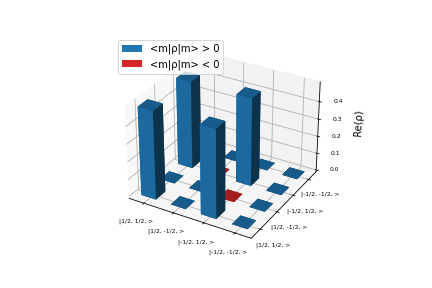
\includegraphics[width=1.5\textwidth]{./spin1-2/33correlated_pure_hyperfine/EvolvedRealPartDensityMatrix.png}
\end{column}
\end{column}
\begin{column}{.5\textwidth}
\includegraphics[width=\textwidth]{./spin1-2/33correlated_pure_hyperfine/FIDSignal.png}
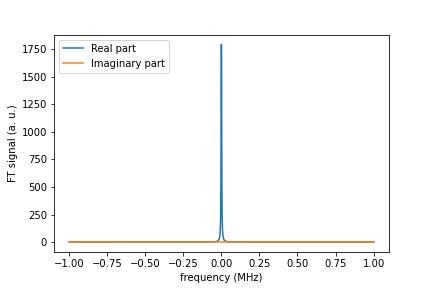
\includegraphics[width=\textwidth]{./spin1-2/33correlated_pure_hyperfine/FTSignal.png}
\end{column}
\end{columns}
\end{frame}
\begin{frame}
\frametitle{32correlated pure dipD2}
Spin: 0.5,$B_0= 10$, $\gamma/2\pi = 4.0$,$\mathcal{H}=\text{I}_{z}+ b_D \big(3\cos^2\theta-1\big)I_{1z}I_{2z}.$$b_D\approx1.571$$theta\approx0.785$
\begin{columns}[T]
\begin{column}{.5\textwidth}
\begin{align*}
\rho_{\text{initial}}\doteq
\begin{pmatrix}
0.5 & 0.0 & 0.5 & 0.0 \\
0.0 & 0.0 & 0.0 & 0.0 \\
0.5 & 0.0 & 0.5 & 0.0 \\
0.0 & 0.0 & 0.0 & 0.0
\end{pmatrix}
\\
\rho_{\text{final}}\doteq
\begin{pmatrix}
0.505 & 0.0 & 0.008 & 0.0 \\
0.0 & 0.0 & 0.0 & 0.0 \\
0.008 & 0.0 & 0.495 & 0.0 \\
0.0 & 0.0 & 0.0 & 0.0
\end{pmatrix}
\end{align*}
\begin{column}{.5\textwidth}
\includegraphics[width=1.5\textwidth]{./spin1-2/32correlated_pure_dipD2/InitialRealPartDensityMatrix.png}
\end{column}
\begin{column}{.5\textwidth}
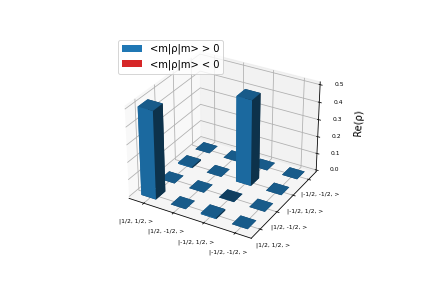
\includegraphics[width=1.5\textwidth]{./spin1-2/32correlated_pure_dipD2/EvolvedRealPartDensityMatrix.png}
\end{column}
\end{column}
\begin{column}{.5\textwidth}
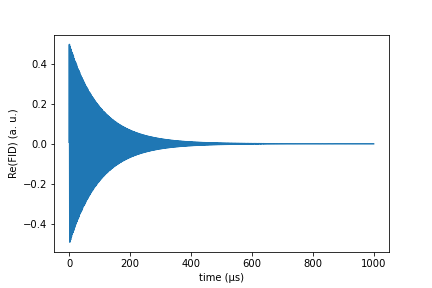
\includegraphics[width=\textwidth]{./spin1-2/32correlated_pure_dipD2/FIDSignal.png}
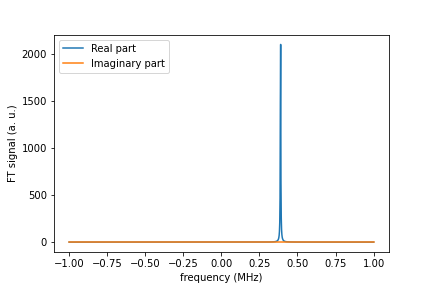
\includegraphics[width=\textwidth]{./spin1-2/32correlated_pure_dipD2/FTSignal.png}
\end{column}
\end{columns}
\end{frame}
\begin{frame}
\frametitle{11uncorrelated mixed no interactions}
Spin: 0.5,$B_0= 10$, $\gamma/2\pi = 4.0$,$\mathcal{H}=\text{I}_{z}$
\begin{columns}[T]
\begin{column}{.5\textwidth}
\begin{align*}
\rho_{\text{initial}}\doteq
\begin{pmatrix}
0.5 & 0.0 & 0.0 & 0.0 \\
0.0 & 0.5 & 0.0 & 0.0 \\
0.0 & 0.0 & 0.0 & 0.0 \\
0.0 & 0.0 & 0.0 & 0.0
\end{pmatrix}
\\
\rho_{\text{final}}\doteq
\begin{pmatrix}
0.5 & 0.0 & 0.004 & 0.0 \\
0.0 & 0.5 & 0.0 & 0.004 \\
0.004 & 0.0 & 0.0 & 0.0 \\
0.0 & 0.004 & 0.0 & 0.0
\end{pmatrix}
\end{align*}
\begin{column}{.5\textwidth}
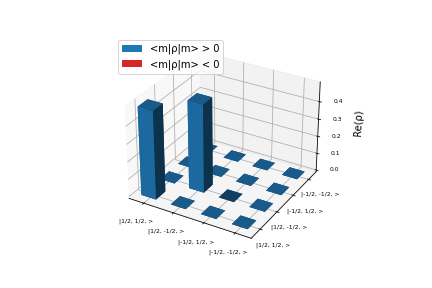
\includegraphics[width=1.5\textwidth]{./spin1-2/11uncorrelated_mixed_no_interactions/InitialRealPartDensityMatrix.png}
\end{column}
\begin{column}{.5\textwidth}
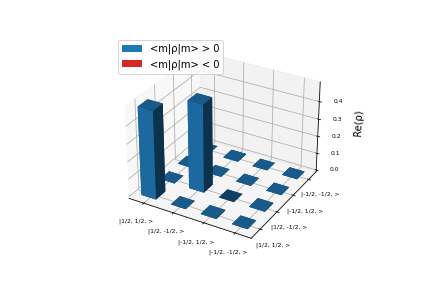
\includegraphics[width=1.5\textwidth]{./spin1-2/11uncorrelated_mixed_no_interactions/EvolvedRealPartDensityMatrix.png}
\end{column}
\end{column}
\begin{column}{.5\textwidth}
\includegraphics[width=\textwidth]{./spin1-2/11uncorrelated_mixed_no_interactions/FIDSignal.png}
\includegraphics[width=\textwidth]{./spin1-2/11uncorrelated_mixed_no_interactions/FTSignal.png}
\end{column}
\end{columns}
\end{frame}
\begin{frame}
\frametitle{41correlated mixed no interaction}
Spin: 0.5,$B_0= 10$, $\gamma/2\pi = 4.0$,$\mathcal{H}=\text{I}_{z}$
\begin{columns}[T]
\begin{column}{.5\textwidth}
\begin{align*}
\rho_{\text{initial}}\doteq
\begin{pmatrix}
0.3 & 0.0 & 0.0 & 0.0 \\
0.0 & 0.3 & 0.0 & 0.0 \\
0.0 & 0.0 & 0.2 & 0.0 \\
0.0 & 0.0 & 0.0 & 0.2
\end{pmatrix}
\\
\rho_{\text{final}}\doteq
\begin{pmatrix}
0.3 & 0.0 & 0.001 & -0.0 \\
0.0 & 0.3 & -0.0 & 0.001 \\
0.001 & -0.0 & 0.2 & 0.0 \\
-0.0 & 0.001 & 0.0 & 0.2
\end{pmatrix}
\end{align*}
\begin{column}{.5\textwidth}
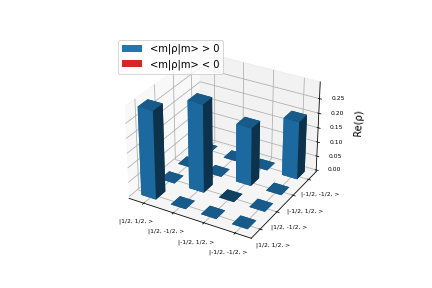
\includegraphics[width=1.5\textwidth]{./spin1-2/41correlated_mixed_no_interaction/InitialRealPartDensityMatrix.png}
\end{column}
\begin{column}{.5\textwidth}
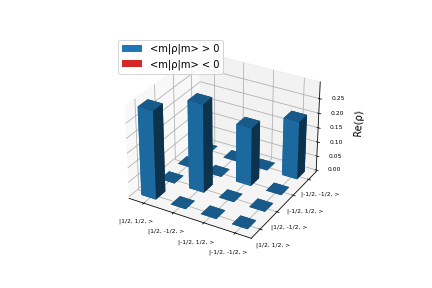
\includegraphics[width=1.5\textwidth]{./spin1-2/41correlated_mixed_no_interaction/EvolvedRealPartDensityMatrix.png}
\end{column}
\end{column}
\begin{column}{.5\textwidth}
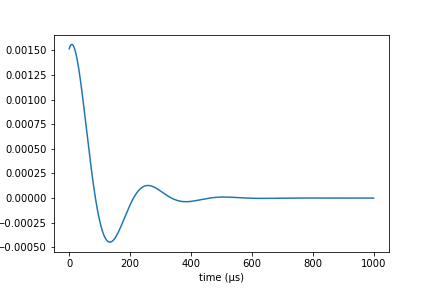
\includegraphics[width=\textwidth]{./spin1-2/41correlated_mixed_no_interaction/FIDSignal.png}
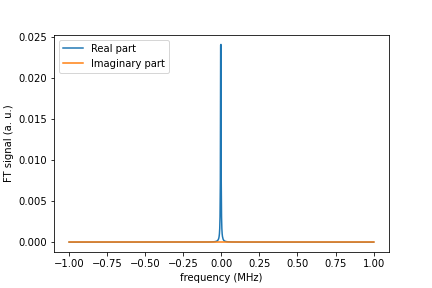
\includegraphics[width=\textwidth]{./spin1-2/41correlated_mixed_no_interaction/FTSignal.png}
\end{column}
\end{columns}
\end{frame}
\begin{frame}
\frametitle{21uncorrelated pure no interactions}
Spin: 0.5,$B_0= 10$, $\gamma/2\pi = 4.0$,$\mathcal{H}=\text{I}_{z}$
\begin{columns}[T]
\begin{column}{.5\textwidth}
\begin{align*}
\rho_{\text{initial}}\doteq
\begin{pmatrix}
1.0 & 0.0 & 0.0 & 0.0 \\
0.0 & 0.0 & 0.0 & 0.0 \\
0.0 & 0.0 & 0.0 & 0.0 \\
0.0 & 0.0 & 0.0 & 0.0
\end{pmatrix}
\\
\rho_{\text{final}}\doteq
\begin{pmatrix}
1.0 & 0.0 & 0.008 & 0.0 \\
0.0 & 0.0 & 0.0 & 0.0 \\
0.008 & 0.0 & 0.0 & 0.0 \\
0.0 & 0.0 & 0.0 & 0.0
\end{pmatrix}
\end{align*}
\begin{column}{.5\textwidth}
\includegraphics[width=1.5\textwidth]{./spin1-2/21uncorrelated_pure_no_interactions/InitialRealPartDensityMatrix.png}
\end{column}
\begin{column}{.5\textwidth}
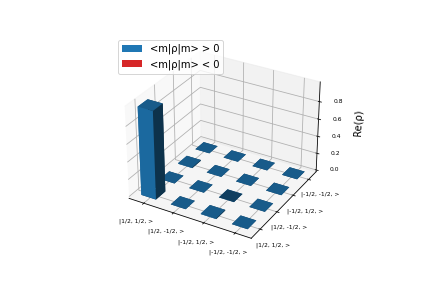
\includegraphics[width=1.5\textwidth]{./spin1-2/21uncorrelated_pure_no_interactions/EvolvedRealPartDensityMatrix.png}
\end{column}
\end{column}
\begin{column}{.5\textwidth}
\includegraphics[width=\textwidth]{./spin1-2/21uncorrelated_pure_no_interactions/FIDSignal.png}
\includegraphics[width=\textwidth]{./spin1-2/21uncorrelated_pure_no_interactions/FTSignal.png}
\end{column}
\end{columns}
\end{frame}
\begin{frame}
\frametitle{34correlated pure hyperfineAnisotrop}
Spin: 0.5,$B_0= 10$, $\gamma/2\pi = 4.0$,$\mathcal{H}=\text{I}_{z}+ \hat{S}\tilde{A}\hat{I}$$A=[[2, 0, 0], [0, 1, 0], [0, 0, 1]]$,
\begin{columns}[T]
\begin{column}{.5\textwidth}
\begin{align*}
\rho_{\text{initial}}\doteq
\begin{pmatrix}
0.5 & 0.0 & 0.5 & 0.0 \\
0.0 & 0.0 & 0.0 & 0.0 \\
0.5 & 0.0 & 0.5 & 0.0 \\
0.0 & 0.0 & 0.0 & 0.0
\end{pmatrix}
\\
\rho_{\text{final}}\doteq
\begin{pmatrix}
0.5 & 0.0 & 0.5 & 0.0 \\
0.0 & 0.0 & -0.0 & 0.0 \\
0.5 & -0.0 & 0.5 & -0.0 \\
0.0 & 0.0 & -0.0 & 0.0
\end{pmatrix}
\end{align*}
\begin{column}{.5\textwidth}
\includegraphics[width=1.5\textwidth]{./spin1-2/34correlated_pure_hyperfineAnisotrop/InitialRealPartDensityMatrix.png}
\end{column}
\begin{column}{.5\textwidth}
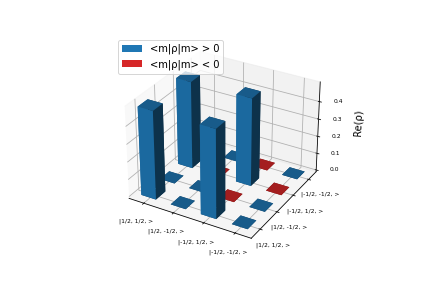
\includegraphics[width=1.5\textwidth]{./spin1-2/34correlated_pure_hyperfineAnisotrop/EvolvedRealPartDensityMatrix.png}
\end{column}
\end{column}
\begin{column}{.5\textwidth}
\includegraphics[width=\textwidth]{./spin1-2/34correlated_pure_hyperfineAnisotrop/FIDSignal.png}
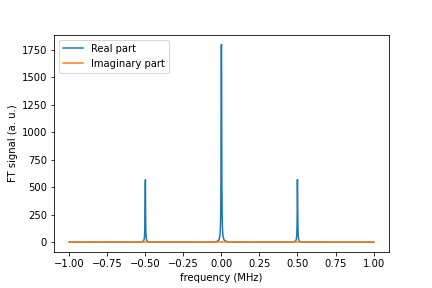
\includegraphics[width=\textwidth]{./spin1-2/34correlated_pure_hyperfineAnisotrop/FTSignal.png}
\end{column}
\end{columns}
\end{frame}
\begin{frame}
\frametitle{23uncorrelated pure hyperfine}
Spin: 0.5,$B_0= 10$, $\gamma/2\pi = 4.0$,$\mathcal{H}=\text{I}_{z}+ \hat{S}\tilde{A}\hat{I}$$A=[[1, 0, 0], [0, 1, 0], [0, 0, 1]]$,
\begin{columns}[T]
\begin{column}{.5\textwidth}
\begin{align*}
\rho_{\text{initial}}\doteq
\begin{pmatrix}
1.0 & 0.0 & 0.0 & 0.0 \\
0.0 & 0.0 & 0.0 & 0.0 \\
0.0 & 0.0 & 0.0 & 0.0 \\
0.0 & 0.0 & 0.0 & 0.0
\end{pmatrix}
\\
\rho_{\text{final}}\doteq
\begin{pmatrix}
1.0 & 0.0 & -0.0 & -0.0 \\
0.0 & 0.0 & 0.0 & 0.0 \\
-0.0 & 0.0 & 0.0 & 0.0 \\
-0.0 & 0.0 & 0.0 & 0.0
\end{pmatrix}
\end{align*}
\begin{column}{.5\textwidth}
\includegraphics[width=1.5\textwidth]{./spin1-2/23uncorrelated_pure_hyperfine/InitialRealPartDensityMatrix.png}
\end{column}
\begin{column}{.5\textwidth}
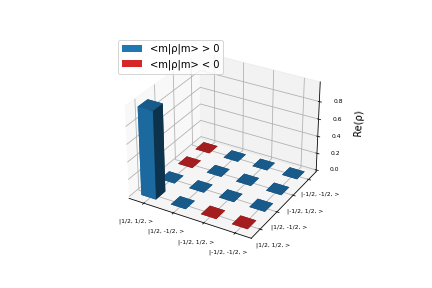
\includegraphics[width=1.5\textwidth]{./spin1-2/23uncorrelated_pure_hyperfine/EvolvedRealPartDensityMatrix.png}
\end{column}
\end{column}
\begin{column}{.5\textwidth}
\includegraphics[width=\textwidth]{./spin1-2/23uncorrelated_pure_hyperfine/FIDSignal.png}
\includegraphics[width=\textwidth]{./spin1-2/23uncorrelated_pure_hyperfine/FTSignal.png}
\end{column}
\end{columns}
\end{frame}
\begin{frame}
\frametitle{24uncorrelated pure hyperfineAnisotrop}
Spin: 0.5,$B_0= 10$, $\gamma/2\pi = 4.0$,$\mathcal{H}=\text{I}_{z}+ \hat{S}\tilde{A}\hat{I}$$A=[[2, 0, 0], [0, 1, 0], [0, 0, 1]]$,
\begin{columns}[T]
\begin{column}{.5\textwidth}
\begin{align*}
\rho_{\text{initial}}\doteq
\begin{pmatrix}
1.0 & 0.0 & 0.0 & 0.0 \\
0.0 & 0.0 & 0.0 & 0.0 \\
0.0 & 0.0 & 0.0 & 0.0 \\
0.0 & 0.0 & 0.0 & 0.0
\end{pmatrix}
\\
\rho_{\text{final}}\doteq
\begin{pmatrix}
1.0 & 0.0 & -0.0 & -0.0 \\
0.0 & 0.0 & 0.0 & -0.0 \\
-0.0 & 0.0 & 0.0 & -0.0 \\
-0.0 & -0.0 & -0.0 & 0.0
\end{pmatrix}
\end{align*}
\begin{column}{.5\textwidth}
\includegraphics[width=1.5\textwidth]{./spin1-2/24uncorrelated_pure_hyperfineAnisotrop/InitialRealPartDensityMatrix.png}
\end{column}
\begin{column}{.5\textwidth}
\includegraphics[width=1.5\textwidth]{./spin1-2/24uncorrelated_pure_hyperfineAnisotrop/EvolvedRealPartDensityMatrix.png}
\end{column}
\end{column}
\begin{column}{.5\textwidth}
\includegraphics[width=\textwidth]{./spin1-2/24uncorrelated_pure_hyperfineAnisotrop/FIDSignal.png}
\includegraphics[width=\textwidth]{./spin1-2/24uncorrelated_pure_hyperfineAnisotrop/FTSignal.png}
\end{column}
\end{columns}
\end{frame}

\end{document}